%-*- mode: LaTex; outline-regexp: "\\\\section\\|\\\\subsection";fill-column: 80; -*-
\documentclass[12pt]{article}
\usepackage[longnamesfirst]{natbib}
\usepackage[usenames]{color}
\usepackage{graphicx}  % Macintosh pdf files for figures
\usepackage{amssymb}   % Real number symbol {\Bbb R}
\input{../../standard}

% --- margins
\usepackage{../sty/simplemargins}
\setleftmargin{1in}   % 1 inch is NSF legal minimum
\setrightmargin{1in}  % 1 inch is NSF legal minimum
\settopmargin{1in}    % 1 inch is NSF legal minimum
\setbottommargin{1in} % 1 inch is NSF legal minimum

% --- Paragraph split, indents
\setlength{\parskip}{0.00in}
\setlength{\parindent}{0in}

% --- Line spacing
\renewcommand{\baselinestretch}{1.5}

% --- page numbers
\pagestyle{empty}  % so no page numbers

% --- Hypthenation
\sloppy  % fewer hyphenated
\hyphenation{stan-dard}
\hyphenation{among}

% --- Customized commands, abbreviations
\newcommand{\TIT}{{\it  {\tiny Featurizing Text (DRAFT, \today)}}}

% --- Header
\pagestyle{myheadings}
\markright{\TIT}

% --- Title

\title{ Featurizing Text: Converting Text into Predictors for
            Regression Analysis }
\author{
        Dean P. Foster\footnote{Research supported by NSF grant 1106743} 
        \ \ Mark Liberman 
        \ \ Robert A. Stine\footnotemark[\value{footnote}]   \\
        Department of Statistics                             \\
        The Wharton School of the University of Pennsylvania \\
        Philadelphia, PA 19104-6340                          
}

\date{\today}

%%%%%%%%%%%%%%%%%%%%%%%%%%%%%%%%%%%%%%%

\begin{document}
\maketitle 
%------------------------------------------------------------------------
\vspace{-.5in}
\abstract{  

 Modern data streams routinely combine text with the familiar numerical data used
 in regression analysis.  For example, listings for real estate that show the price
 of a property typically include a verbal description.  Some 
 descriptions include numerical data, such as the number of rooms or the size of
 the home.  Many others, however, only verbally describe the property, often
 using an idiosyncratic vernacular.  For modeling such data, we describe several methods that that convert such text into numerical features
 suitable for regression analysis.  The proposed featurizing techniques create
 regressors directly from text, requiring minimal user input.  The techniques range naive to subtle.  One can simply use raw counts of words, obtain principal components from these counts, or build regressors from counts of  adjacent words.  Our example that models real estate prices illustrates the surprising success of these methods.  To partially explain this success, we offer a motivating probabilistic model.  Because the derived regressors are difficult to interpret, we further show how the presence of  partial quantitative features extracted from text can elucidate the structure of a model.

}

%------------------------------------------------------------------------
\vspace{0.05in}

\noindent
{\it Key Phrases: sentiment analysis, n-gram, latent semantic analysis } 

\clearpage

% To Do
% 

% ----------------------------------------------------------------------
\section{Introduction}
% ----------------------------------------------------------------------

 Modern data streams routinely combine text with numerical data suitable for in
 regression analysis.  For example, patient medical records combine lab
 measurements with physician comments and online product ratings such as those
 at Amazon or Netflix blend explicit characteristics with verbal commentary. As
 a specific example, we build a regression model to predict the price of real
 estate from its listing.  The listings we use are verbal rather than
 numerical data obtained by filling out a spreadsheet-like form.  Here are four
 such listings for Chicago, IL, extracted (with permission) from trulia.com on June 12, 2013:

 \begin{verbatim}
    $399000 Stunning skyline views like something from a postcard are yours
    with this large 2 bed, 2 bath loft in Dearborn Tower!  Detailed
    hrdwd floors throughout the unit compliment an open kitchen and
    spacious living-room and dining-room /w walk-in closet, steam
    shower and marble entry.  Parking available. 

    $13000 4 bedroom, 2 bath 2 story frame home. Property features a
    large kitchen, living-room and a full basement. This is a Fannie Mae
    Homepath property. 

    $65000 Great short sale opportunity...  Brick 2 flat with 3 bdrm
    each unit. 4 or more cars parking. Easy to show. 

    $29900 This 3 flat with all 3 bed units is truly a great
    investment!! This property also comes with a full attic that has
    the potential of a build-out-thats a possible 4 unit building in a 
    great area!!  Blocks from lake and transportation. Looking for a
    deal in todays market - here is the one!!! 
 \end{verbatim}

 \noindent
 The only numerical data common to the listings is the price that appears at
 the head of each listing.  Some listings include further numerical data, such
 as the number of rooms or occasionally the size of the property (number of
 square feet).  Many listings, however, provide only a verbal description,
 often written in an idiosyncratic vernacular familiar only to those who are
 house hunting. Some authors write in sentences, others not, and a variety of
 abbreviations appear.  The style of punctuation varies from spartan to effusive
 (particularly exclamation marks), and the length of the listing runs from
 several words to a long paragraph.

 
 An obvious approach to building regressors from text data relies on a
 substantive analysis of the text.  For example, sentiment analysis constructs a
 domain-specific lexicon of positive and negative words.  In the context of real
 estate, words such as `modern' and `spacious' might be flagged as positive
 indicators (and so be associated with more expensive properties), whereas
 `Fannie Mae' and `fixer-upper' would be marked as negative indicators.  The
 development of such lexicons has been an active area of research in sentiment
 analysis over the past decade \citep{taboada11}.  The development of a lexicon
 require substantial knowledge of the context and the results are known to be
 domain specific.  Each new problem requires a new lexicon.  The lexicon for
 pricing homes would be quite different from the lexicon for diagnosing patient
 health.  Our approach is also domain specific, but requires little user input
 and so can be highly automated.


 In contrast to substantively oriented modeling, we propose a version of supervised
 sentiment analysis that converts text into conventional explanatory variables.
 We convert the text into conventional numerical regressors (featurize) by exploiting methods from computational linguistics that are familiar to statisticians. These so-called vector space models \citep{turney10}, such as latent semantic analysis (LSA), make use of  singular value decompositions of  the bag-of-words and bigram representations of text. (This connection leads to methods being described as a `spectral algorithm for'.) These representations map words into points in a vector space defined by counts. This approach is highly automated with little need for human intervention, though it makes it easy to exploit such investments when available.  The derived regressors can be used alone or in combination with traditional variables, such as those obtained from a lexicon or other semantic model.  We use the example of real estate listings to illustrate the impact of various  choices on the predictive accuracy.  For example, a regression using the
 automated features produced by this analysis explains over two-thirds of the
 variation in listed prices for real estate in Chicago.  The addition of several
 substantively derived variables adds little.  Though we do not emphasize its
 use here, variable selection can be employed to reduce the ensemble of
 regressors without sacrificing predictive accuracy.


 Our emphasis on predictive accuracy does not necessarily produce an
 interpretable model, and one can use other data to create such structure.  Our
 explanatory variable resemble those from principal components analysis and
 share their anonymity.  To provide more interpretable regressors, the presence
 of partial quantitative information in real estate listings (\eg, some listings
 include the number of square feet) provides what we call ‘lighthouse variables’
 that can be used to derive more interpretable variables.  In our sample, few
 listings (about 6\%) indicate the number of square feet.  With so much missing
 data, this manually derived predictor is not very useful as an explanatory
 variable in a regression.  This partially observed variable can then be used to
 define a weighted sum of the anonymous text-derived features, producing a
 regressor that is both complete (no missing cases) and interpretable.  One
 could similarly use features from a lexicon to provide more interpretable
 features.


 The remainder of this paper develops as follows.  The following section
 provides a concise summary of our technique.  The method is remarkably simple
 to describe.  Section 3 demonstrates the technique using about 7,500 real
 estate listings from Chicago.  Though simple to describe, it is more subtle to
 appreciate why it works.  Our explanation appears in Section \ref{sec:model} which shows how this technique discovers the latent effects in a topic model for text.  We return to models for real estate in Section \ref{sec:cv} with a discussion of the use of variable selection methods ands use cross-validation to measure the success of methods and to compare several models.  Variable selection is particularly relevant if one chooses to search for nonlinear behavior.  Section \ref{sec:light} considers the use of partial semantic information for producing more interpretable models.  We close in Section \ref{sec:disc} with a discussion and collection of future projects.  Our aim is to show how easily one can convert text into familiar regressors for regression.  As such, we leave to others the task of attempting to explain why such simple representations as the co-occurrence of words in documents might capture the deeper meaning  \citep{deerwester90, landauer97, bullinaria07, turney10}. 


%--------------------------------------------------------------------------
\section{An Algorithm for Featurizing Text}
\label{sec:algo}
%--------------------------------------------------------------------------

 Our technique for featurizing text has 3 main steps.  These steps are
 remarkably simple:
 \begin{enumerate}
   \item Convert the source text into lists of word types.  A word type is a
 unique sequence of non-blank characters.  Word types are not distinguished by meaning or use.  That is, this analysis does not distinguish homographs.
   \item Compute matrices that (a) count the number of times that word types
 appear within each document (such as a real estate listing) and (b) count the number of times that word types are found adjacent to each other.
   \item Compute truncated singular value decompositions (SVD) of the resulting
 matrices of counts. The leading singular vectors of these decompositions are our regressors.
 \end{enumerate}
   The simplicity of this approach means that this algorithm runs quickly.  The following analysis of 7,500 real-estate listings generates 1,000 features from raw text in a few seconds on a laptop.  The following paragraphs define our notation and detail what happens within each step. 


 The process of converting the source text into word tokens, known as
 tokenization, is an easily overlooked, but critical step in the analysis.  A
 word token is an instance of a word type, which is roughly a unique sequence of characters delimited by white space.  We adopt a fairly standard, simple approach to converting text into tokens.  We convert all text to lower case, separate punctuation, and replace rare words by an invariant "unknown" token.   To illustrate some of the issues in converting text into tokens, the following string is a portion of the description of a property in Chicago:
 \begin{verbatim}
   Brick flat, 2 bdrm.  With two-car garage. \end{verbatim} 
 \noindent
 Separated into tokens, this text becomes a list of 12 tokens representing 11
 types:
 \begin{verbatim}
   {brick, flat, <,>, 2, bdrm, <.>, with, two, <->, car, garage,<.>} \end{verbatim} 
 \noindent
 \ras{is that what we'd do for the `two-car' item???}
 Once tokenized, all characters are lower case.  Punctuation
 symbols, such as commas and periods, are ``words'' in this sense.  Since little
 is known about rare words that are observed in only one or two documents, we
 represent their occurrence by the symbol `$<$UNK$>$'.  The end of each document is marked by a unique type.  We make no attempt to correct spelling errors and typos nor to expand abbreviations. References such as the books \citet{manning99} and \citet{jurafsky09} describe further processing, such as stemming and annotation that can be done prior to statistical modeling. \citet{turney10} gives a concise overview.
 

Once the source text has been tokenized, we form two matrices of counts.  The SVD of each of these defines a set of explanatory variables.  The matrices, $W$ and $B$,  differ in how they measure the similarity of words. Words are judged to be similar if they appear in the same context.  For the document/word matrix $W$, the context is a document -- a real estate listing.  This matrix holds counts of which words appear in the same document, ignoring the order in which the words appear. This approach treats each document (or listing) as a bag of words, a multiset that does not distinguish the placement of the words.  The second matrix adopts a very different perspective that relies entirely upon ordering; it defines the context by adjacency.  The bigram matrix $B$ counts how often words  appear adjacent to each other.  The document/word and bigram matrices thus represent two extremes of a common approach:  Associate words that co-occur within some context.  $W$ uses the wide window provided by a document, whereas $B$ uses the most narrow window possible. The wider window afforded by a document hints that $W$ emphasizes semantic similarity, whereas the narrow window of adjacency that defines $B$ suggests more emphasis on local syntax.  Curiously, we find either approach effective and make use of both.
 
 
Associating words that co-occur in a document is more familiar to statisticians, and so we begin there.  Let $V$ denote a vocabulary consisting of $M$ unique word types.  The vector $w_i$ holds the counts of these word types for the $i$th document; $w_{im}$ is the number of times word type $m$ appears within the $i$th document.  (All vectors in our notation are column vectors.)  Let $n$ denote the number of documents; these documents are the observational units in our analysis.  Fro models of real estate, a document is the description found in a listing.  We collect the word counts for documents as rows within the $n \times M$ matrix $W$,
 \begin{displaymath}
    W = \left( \begin{array}{c}
                 w_1' \cr w_2' \cr \vdots \cr w_n'
        \end{array} \right)
 \end{displaymath}
 (Note that within computational linguistics it is common to find the transpose of this matrix.)  The matrix $W$ is quite sparse: most documents use a small portion of the  vocabulary.   Let $m_i = \sum_m w_{im}$ denote the number of word tokens that appear in the description of the $i$th property.  It is common within linguistics to transform these counts prior to additional modeling.  For example, the counts might be normalized by document, or transformed to emphasize relatively rare events. \citet{turney10} summarizes several approaches, such as the popular TF-IDF (term frequency-inverse document frequency) and entropy-based transformations.  
 
 
 The bigram matrix counts how often word types occur adjacent to each other.
  Let $B$ define the $M \times M$ matrix produced from the sequence of tokens
 for all documents combined (the corpus).  $B_{ij}$ counts how often word-type
 $i$ precedes work-type $j$ within the corpus.  Whereas $W$ ignores word
 placement (sequencing) within a document, $B$ combines counts over all documents and relies on the sequence of word tokens.


 We obtain regression features from the SVD of $W$ and $B$.  The regressors are immediate from the SVD of $W$.    Let
 \begin{equation}
     W = \tilde{U}_W \tilde{D}_W \tilde{V}_W'   
 \label{eq:svdW}
 \end{equation}
 denote the SVD of $W$. We typically use only a subset of this decomposition, and so  we define $U_W$ to be the $n \times k_W$ matrix defined by the leading $k_W$ singular vectors of $W$ (\ie, the first $k_W$ columns of $\tilde{U}_W$ that are associated with the largest singular values).  The collection $U_W$ defines a collection of regressors.  (The resulting computation that isolates only these leading singular vectors is sometimes called a truncated SVD.)  This representation of text is known as latent semantic analysis (or latent semantic indexing) within computational linguistics; statisticians will recognize this as a principal components analysis (PCA) of $W$.   The choice of the number of singular vectors to retain, $k_W$, is a user-controlled tuning parameter of this technique.  We will provide some advice on unsupervised methods for picking $k_W$ in the following section within the example that analyzes real estate listings in Chicago.  

 
 A second application of the SVD produces regressors from the bigram matrix $B$.
  Let
 \begin{equation}
       B = \tilde{U}_B \tilde{D}_B \tilde{V}_B'
 \label{eq:svdB}
 \end{equation}
 define the SVD of $B$, and again use matrices without $\sim$ to denote components of the truncated SVD:  $U_B$ and $V_B$ denote the first $k_B$ columns of $\tilde{U}_B$ and $\tilde{V}_B$, respectively.  As in the
 decomposition of $W$, the number of singular vector to retain is a user-defined choice.  We generally keep $k_W = k_B$.  Because $B$ is $M
 \times M$, these singular vectors define points in $\R^M$ and are sometimes referred to as ``eigenwords'' because of the way in which they form directions in word space \ras{cite}.  The $i$th row of $U_B$  locates the word type $w_i$ within $\R^{k_B}$  (all of the following applies  to $V_B$ as well).  To build regressors, we locate each document at a point within this same space.  We can think of this location in two, nearly equivalent ways that emphasize either the rows or columns of $U_B$.  The two methods differ in a sum is normalized.  The row-oriented motivation is particularly simple: a document is positioned at the average of the positions of its words.  For example, the $i$th document is located at $w_i'U_B/m_i$.  Alternatively, emphasizing columns, we can compute the correlation between the columns of $U_B$ with the bag-of-words representations of the documents.  Because the columns of $U_B$  and $V_B$ are orthonormal, these correlations are given by
 \begin{equation}
     C = [C_l C_r] 
         = \mbox{diag}(\norm{w_i}^{-1})W[U_B \; V_B]   \;, 
            \quad \mbox{ where } \quad  \normsq{x} = \sum x_i^2  \;.
 \label{eq:C}
 \end{equation}
 The $i$th row of of the $n \times 2k_B$ matrix $C$ is the vector of correlations between the bag-of-words representation $w_i$ and the singular vectors of $B$.  In our models for real-estate listings, the columns of $C$ form the second bundle of regressors.


 It is worthwhile to take note of two properties of these calculations that are
 important in practice.  First, one needs to take advantage of sparsity in the
 matrices $W$ and $B$ to reduce memory usage and to increase the speed of
 computing matrix products.  Second, the computation of the SVD of a large
 matrix can be quite slow.  For example, computing the SVD of $B$ is of order
 $O(M^3)$ and one can easily have vocabulary of $M=$10,000 or more word types.
  To speed this calculation, we exploit random projection algorithms defined and
 analyzed in \citet{tropp10}.


%--------------------------------------------------------------------------
\section{Predicting Prices of Real Estate}
%--------------------------------------------------------------------------

 This section demonstrates the use of regressors defined from text using the
 featurizing techniques defined in the prior section.  The data are $n=$7,384 property listings for Chicago, IL in June, 2013.   (Note that at the time, trulia.com showed  30,322 listings for Chicago, but most of these were foreclosures that are excluded in our analysis.) The response in our models is the log of the listed price.  The prices for properties listed in Chicago is quite skewed, so we transformed the response to a log scale as shown in the histogram of Figure \ref{fig:prices}.  This display uses the base 10 log of the prices for easy interpretation; subsequent models use natural logs throughout.  The log
 transformation produces a roughly Gaussian distribution, with a hint of fat
 tails most prominently for cheaper properties with prices near \$25,000.


 \begin{figure}
 \caption{ \label{fig:prices} { \sl The distribution of prices for real estate
 in Chicago is highly skewed, but a log transformation produces data that are
 nearly normal.} The presence of a long lower tail might indicate that the data
 mix typical home sales with special, subsided properties or perhaps vacant lots
 that sell for an unusually low price. }

 \centerline{
 \vspace{0.1in}
 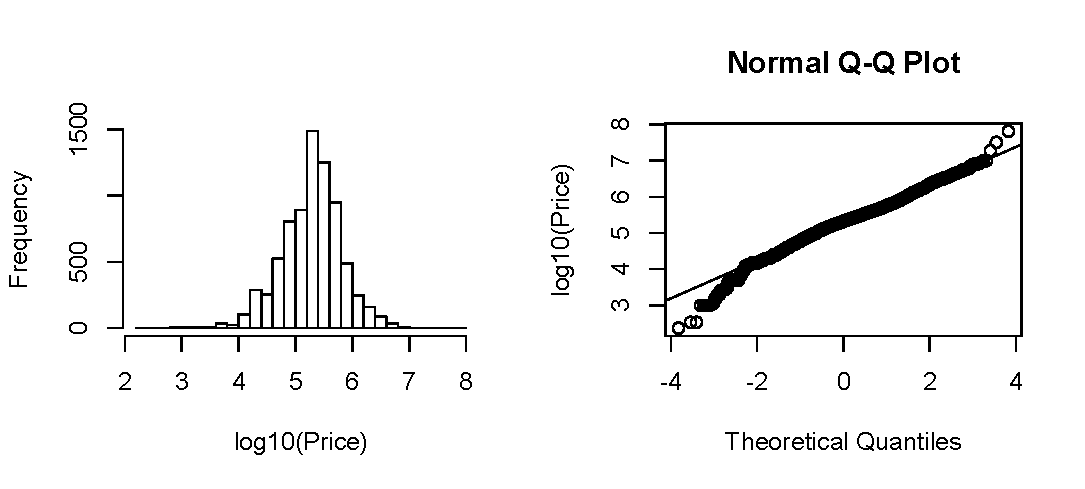
\includegraphics[width=5in]{figures/prices} }
 \vspace{0.2in}
 \end{figure}


 \subsection{ Tokenization and Parsing }

 The 7,384 property listings in Chicago contain 543,869 word tokens that define
 15,228 word types.  More than half of these tokens appear only once or twice,
 providing little exposure to how the word is used.  We clustered these
 rare types into one category ($<$UNK$>$), resulting in a reduced vocabulary of
 $M = 5,708$ word types.  The most common word types are ``not words'' but
 rather punctuation: `.'  occurs 40,227 times and `,' 33,746 times.  Following
 these come the collection of seldom seen words (OOV, 11,478), `and' (frequency 11,032), `!' (7,894) and `in' (7,418).    As usual in text, ``most types are common but most words are rare.''  That is, the most common types occur frequently whereas most words appear infrequently.  Figure \ref{fig:zipf} shows a scatterplot of the log of the frequency of these word types versus the log of their ranks.  It is common in text to find a linear trend with slope near 1 in this graph, a Zipf distribution \citep{zipf35, baayen02}.  Even though this text is not standard English, one expects to find counts resembling those produced by a power law \citep{clauset09}.  For
 this text, the shown line (with log-log slope -0.927) holds only for more
 common word types.  For less common words (here, outside the most common 500
 words), the frequencies drop off more rapidly.  (This change in slope is also
 seen for words in Wikipedia.)


 \begin{figure}
 \caption{ \label{fig:zipf} { \sl The log of the frequency of word types in the
 listings for properties in Chicago is roughly linear in the log of the rank of
 the words, a Zipf distribution.}  The shown line $\log \mbox{freq} = 10.9 -
 0.93 \log \mbox{rank}$ was fit to words with ranks 1 through 500.  }

 \centerline{
 \vspace{0.1in}
 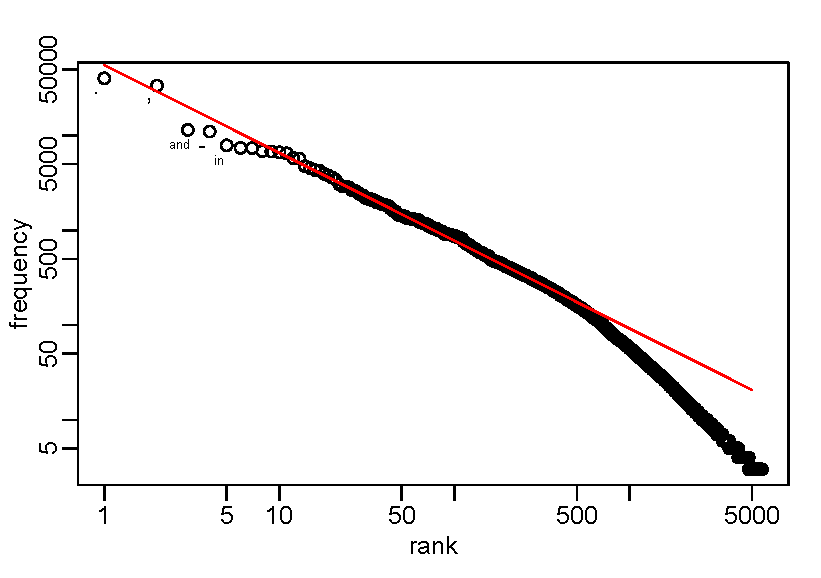
\includegraphics[width=3.5in]{figures/zipf} }
 \vspace{0.2in}
 \end{figure}


 The average description has about 73 word tokens, but the distribution of the
 lengths $m_i$ is right skewed.  The boxplot in Figure \ref{fig:boxplot} shows
 the lengths.  The shortest description has 2 tokens, whereas the longest
 description has 568 tokens.  This variation in the lengths of the descriptions
 suggests that modeling the prices from this text will require a weighted
 regression.  We simply do not know so much about  properties with short
 descriptions.


 \begin{figure}
 \caption{ \label{fig:boxplot} { \sl The distribution of the lengths $m_i$ of
the property descriptions is right-skewed, with some listing running hundreds of
words compared to a median length of 74 words. } }

 \centerline{
 \vspace{0.1in}
 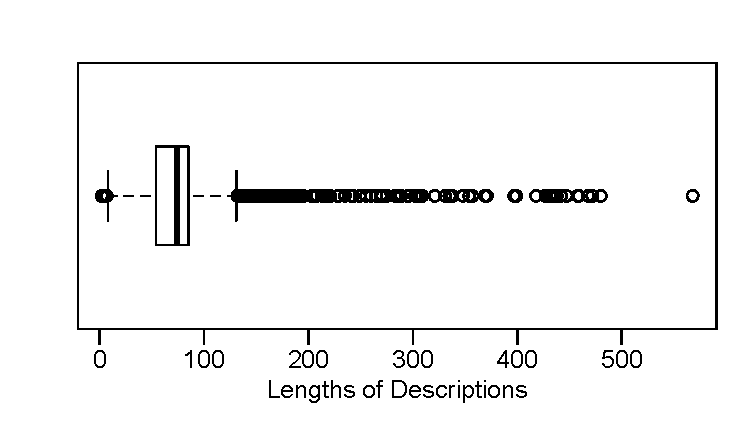
\includegraphics[width=3.5in]{figures/boxplot} }
 \vspace{0.2in}
 \end{figure}


 Before we use the decomposition rules to construct regressions, we construct
 several by extracting explicit values from the descriptions.  For example when
 processing ads for real estate, one might conjecture that an agent has a lot
 more to say in when describing the features of an expensive property than a
 property in need of repair, implying that the length of the ad for a property
 would $m_i$ may be predictive of the price.  In addition, one can use a regular
 expression to extract the number of bedrooms when it appears in the listing.
  We wrote regular expressions to extract numerical data from advertisements
 when present.  Constructing these is a labor-intensive process that must be
 done on a case-by-case basis.  For example, a regular expression would parse
 the value 2 for the number of bedrooms and bathrooms from the first listing
 shown in the introduction.  The patterns used in these regular expressions
 allow common abbreviations, such as ``bth'', ``bath'' and ``bthrm'' for
 bathrooms.  Another regular expression that we used extracts the number of
 square feet from the listing.  Most listings, however, omit these
 characteristics.  For Chicago, our regular expressions found that 6\% of the
 listings indicate the number of square feet, 26\% indicate the number of
 bathrooms, and 42\% give the number of bedrooms.  More complex regular
 expressions would likely find more matches, but the gains are likely to be few.
  One also faces a Type I/Type II trade-off.  Simple regular
 expressions omit some matches, but more aggressive expressions 
 match inadvertently.  To accommodate the large amount of missing data, we used
 the simple procedure of adding indicator variables that distinguish observed
 cases for these variables, and we then filled the missing values with means.


 The four scatterplots in Figure \ref{fig:parsed} summarize the marginal
 association between the log of prices and these parsed predictors, including
 the number of words in descriptions.  Missing values produce the columns of
 gray points located at the mean of the variable on the $x$ axis.  None of these
 features is highly correlated with the log of price; the highest correlations
 are with the length of the description ($r=0.40$) and the number of bathrooms
 ($r = 0.19$).  One explanation for the low association is the abundance of
 missing data.  For example, corr(log price, log sq ft) $= 0.00$ overall, but is
  larger (0.26) among the few properties that report this characteristic.
  These plots also show several  anomalies.  For example, the first
 scatterplot of the log of price on the number of words shows a cluster of
 25 listings, all with exactly 265 words.  All of these different properties were listed in a common format by a government agency.   The scatterplot of the log of prices
 on the log of the square footage also shows a clear outlier; this outlier is a
 consequence of aggressive parsing.  A typo in a description (``has 1sfam'') led to  
 the regular expression finding a property with 1 square foot.

 \begin{figure}
  \caption{ \label{fig:parsed} { \sl The parsed characteristics have slight
 positive association with the log of the prices. } Gray points in the figures
 identify cases that were missing the explanatory variable; the shown
 correlation uses the complete, filled-in data. }

 \centerline{
 \vspace{0.1in}
 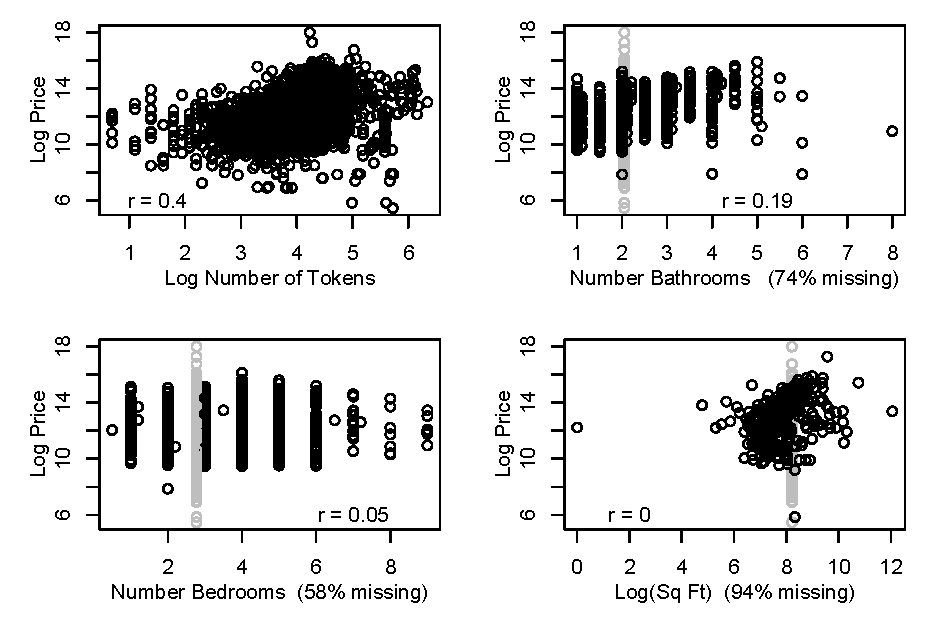
\includegraphics[width=5in]{figures/parsed} }
 \vspace{0.2in}
 \end{figure}


 Table \ref{tab:parsed} summarizes the fit of the regression of the log of price
 on these four extracted variables and the missing indicators.   In this first example, the regressors are not highly correlated, and the importance of these variables in the multiple regression generally echoes the marginal correlations shown in Figure \ref{fig:parsed}.  Among the seven explanatory variables, the length of the descriptions is most predictive, followed by the number of bathrooms.  Unlike the marginal associations, however, both the log of the number of square feet (when observed) and its missing indicator are significant.  The missing indicators for bedrooms and bathrooms are not predictive.  The model
 obtains adjusted R-squared $\ol{R}^2 = 0.192$, with residual standard deviation $s_e =1.08$.  Because we compare regression models with varying numbers of explanatory variables, $\ol{R}^2$ is more useful than without adjusting for degrees of freedom.  Since
 we are not doing variable selection at this point, but rather fitting full ensembles of
 pre-selected variables, adjusted R-squared is an unbiased summary of each
 model's performance out of sample.  (Section \ref{sec:cv} reports cross-validation results for these models.) 


 \begin{table}
 \caption{ \label{tab:parsed} {\sl OLS multiple regression of log prices on the
 parsed explanatory variables and  indicators of observed values.}}

\begin{center}
\begin{tabular}{rrrrr}
  \hline
 & Estimate & Std. Error & t value & Pr($>$$|$t$|$) \\ 
  \hline
 Intercept & 4.8858 & 0.4944 & 9.88 & 0.0000 \\ 
  $\log m$ & 0.8211 & 0.0239 & 34.31 & 0.0000 \\ 
  log Sq Ft & 0.3680 & 0.0592 & 6.21 & 0.0000 \\ 
  Sq Ft Obs & 0.6108 & 0.0607 & 10.06 & 0.0000 \\ 
  Bedrooms & -0.0095 & 0.0169 & -0.56 & 0.5734 \\ 
  Bedroom Obs & 0.0023 & 0.0306 & 0.08 & 0.9400 \\ 
  Bathrooms & 0.4153 & 0.0307 & 13.53 & 0.0000 \\ 
  Bathroom Obs & 0.0038 & 0.0344 & 0.11 & 0.9127 \\ 
   \hline
\end{tabular}

   $s_e = 1.084$ with $R^2= 0.193,\;	\ol{R}^2 = 0.192$ 
 \end{center}
\end{table}


Before building models using singular vectors, we begin by regressing the response on indicators for the words.  That is, we simply regress $y$ on the word counts in $W$.  This model provides a baseline for comparison with the fits produced by regressions using singular vectors.  Table \ref{tab:regrInd} summarizes the fit using the most common 2,000 words.  Overall, this model produces $\ol{R}^2 = 0.681$.  Residual plots show fat tails (consistent with that in the prices, Figure \ref{fig:prices}) but no clear evidence of heteroscedasticity that might be anticipated due to the differences in the document lengths (Figure \ref{fig:boxplot}).  The most significant word is ``vacant'' with $t=-8.5$; not surprisinging, the presence of this word in a listing indicates a property with lower than usual value.  In contrast, out-of-vocabulary words denoted ``OOV'' have higher than average prices ($t=6.3$). Figure \ref{fig:regrInd} summarizes the distribution of all t-statistics in this model.  Twenty-two words are not used due to singularities among these counts, leaving 1,978 estimated coefficients.  The dashed line in the scatterplot of $|t_j|$ on $j$ in the left panel of Figure \ref{fig:regrInd} is the Bonferroni threshold $\Phi^{-1}(1-0.025/1978) \approx 4.21$.  Only 14 estimates exceed this threshold for statistical significance.  The nearly flat red line in the figure is a lowess smooth of the $|t_j|$.  The half-normal plot in the right panel of Figure \ref{fig:regrInd} confirms the diffuse signal in this model: the distribution of the fitted $t$-statistics is not far from the null distribution.  The gray line in the half-normal plot is the diagonal; the red line is the fitted regression of the smallest 200  $|t|$-statistics on the corresponding quantiles.  For a sample from a standard normal distribution, the slope of a line fit to the $t$ values should be 1.  The slope of the fitted line for these estimates is significantly larger, but clearly the signal is widely spread over these estimates.  A regression on counts for 14 words whose estimates exceed the Bonferroni bound (Table \ref{tab:regrInd}) obtains $\ol{R}^2 = 0.191$.  \ras{Thus, this estimation problem differs from the so-called ``nearly black'' models often studied in research on variable selection.  In those models, a few estimates stand out from a noisy background. In this application, much of the signal lies embedded in that background.}

 \begin{table}
 \caption{ \label{tab:regrInd} {\sl Multiple regression of log prices on 
  counts from the document/word matrix $W$ for the most common 2,000 words.}  The table shows the 14 estimates that exceed the Bonferroni threshold for statistical significance.} 

\begin{center}
\begin{tabular}{rrrrr}
  \hline
 & Estimate & Std. Error & $t$ & Pr($>|t|$) \\ 
  \hline
  vacant & -0.5518 & 0.0652 & -8.46 & 0.0000 \\ 
  deed & -1.3155 & 0.1557 & -8.45 & 0.0000 \\ 
  OOV & 0.0373 & 0.0059 & 6.33 & 0.0000 \\ 
  units & 0.1929 & 0.0342 & 5.64 & 0.0000 \\ 
  discount & -1.4959 & 0.2992 & -5.00 & 0.0000 \\ 
  investment & -0.2334 & 0.0497 & -4.70 & 0.0000 \\ 
  most & 0.3350 & 0.0736 & 4.55 & 0.0000 \\ 
  bucktown & 0.3570 & 0.0790 & 4.52 & 0.0000 \\ 
  sf & 0.3305 & 0.0741 & 4.46 & 0.0000 \\ 
  pullman & -0.6244 & 0.1423 & -4.39 & 0.0000 \\ 
  bedroom & -0.0978 & 0.0227 & -4.31 & 0.0000 \\ 
  terraces & 0.7074 & 0.1650 & 4.29 & 0.0000 \\ 
  fenced & -0.2466 & 0.0578 & -4.27 & 0.0000 \\ 
  scb & -5.5914 & 1.3244 & -4.22 & 0.0000 \\ 
 \hline
\end{tabular}
 
    $s_e =  0.682$ with $R^2 =  0.766$, $\ol{R}^2 =  0.681$  
\end{center}
\end{table}


\ras{Add line at sqrt(2/pi) to left hand figure.}


 \begin{figure}
  \caption{ \label{fig:regrInd} { \sl Distribution of the t-statistics for the regression of log prices on 2,000 word indicators (columns of $W$).}}
 \centerline{  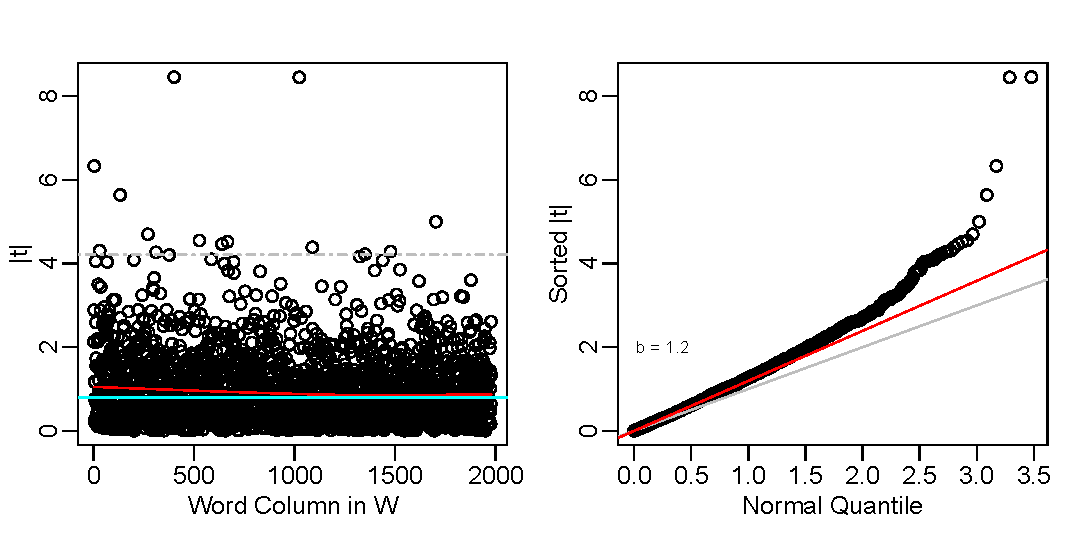
\includegraphics[width=6in]{figures/tstatRegrInd}    }
 \vspace{0.2in}
 \end{figure}

 
 The next model uses regressors created from the SVD of the document/word
 count matrix $W$ defined in equation \eqn{eq:svdW}.  We retained $k_W = 100,\, 200, \, \ldots, 500$ singular vectors of $W$.   Our analysis suggests each of these collections of singular vectors both retains too many insignificant features while at the same time omits others that are predictive.  Broadly speaking, the leading singular vectors (those with larger singular values) are more predictive than subsequent singular vectors.  That said, not all of the leading vectors are statistically significant nor do all of the later singular vectors have coefficients near zero.   As a result, variable selection from a yet larger collection of singular vectors may provide a better fit, a task we defer to Section \ref{sec:cv}.  
 

Each collection of singular vectors explains more variation than the simple model derived from several parsed words, but none find all of the signal captured by the larger collection of 2,000 word indicators.  A regression of log prices on the 100 leading singular vectors attains $\ol{R}^2 = 0.49$, more than twice that of the model with parsed variables.  Adding more singular vectors produces statistically significant, though diminishing improvements.  The collection of 500 singular vectors of $W$ produces $\ol{R}^2 = 0.61$, which is less than the $\ol{R}^2 = 0.68$ derived from individual word counts.  Table \ref{tab:regrW}  shows several of the estimated coefficients and summarizes the overall fits of these models.  As often seen in principal components regression, the statistical significance of the singular vectors is not monotonic in the order of the singular vectors. That said, the leading singular vectors tend to be more relevant than those that follow. Figure \ref{fig:svdregr} summarizes the significance of the estimated coefficients in the same fashion as Figure \ref{fig:regrInd} with a plot of the absolute $t$-statistics and a half-normal plot. Most of the main leading singular vectors are significant, with an increasing proportion of insignificant variables as the position in the decomposition increases.  In comparison to the significance for the coefficients of the word indicators, these singular vectors by-and-large are more consistently predictive with less noise.  The slope of the fit in the half-normal plot (using the least significant 200 estimates) is 2.9.  Residual analysis again finds fat tails with only a hint of heteroscedasticity.
 
 
 Not only can one continue to add further singular vectors, one can also consider nonlinearities in the form of interactions among these singular vectors.  The addition of interactions improves the fit of this model immensely by taking advantage of nonlinearities (\ie, synergies among the eigenword structure).  For example, a regression using just the first 20 singular vectors of $W$ obtains $\ol{R}^2 = 0.31$.  Adding interactions among these (an additional 190 explanatory variables since no powers are added) improves the fit significantly to $\ol{R}^2 = 0.41$.  Fitting models with interactions drawn from a larger collection of features more generally requires some form of selection or regularization.  We pursue this further in Section \ref{sec:cv}.
 

 \begin{table}
 \caption{ \label{tab:regrW} {\sl Multiple regression of log prices on
  singular vectors of the document/word count matrix $W$.}  The first table shows estimated coefficients for first 10 and last 3 singular vectors with $k_w = 500$.  }

\begin{center}
\begin{tabular}{rrrrr}
  \hline
 & Estimate & Std. Error & t value & Pr($>$$|$t$|$) \\ 
  \hline
  D1 & -62.0847 & 2.4891 & -24.94 & 0.0000 \\ 
  D2 & -7.6494 & 0.9373 & -8.16 & 0.0000 \\ 
  D3 & -12.5468 & 0.7558 & -16.60 & 0.0000 \\ 
  D4 & 10.4948 & 0.8262 & 12.70 & 0.0000 \\ 
  D5 & -0.8683 & 0.7645 & -1.14 & 0.2561 \\ 
  D6 & 7.6848 & 0.8036 & 9.56 & 0.0000 \\ 
  D7 & -17.8753 & 0.7547 & -23.69 & 0.0000 \\ 
  D8 & 18.8346 & 0.7577 & 24.86 & 0.0000 \\ 
  D9 & 3.9515 & 0.7540 & 5.24 & 0.0000 \\ 
  D10 & 4.0974 & 0.7521 & 5.45 & 0.0000 \\  
  $\vdots$ & & & & \\
  D498 & 1.2327 & 0.7516 & 1.64 & 0.1010 \\ 
  D499 & 1.3265 & 0.7516 & 1.76 & 0.0776 \\ 
  D500 & 2.5296 & 0.7516 & 3.37 & 0.0008 \\ 
   \hline
\end{tabular}
\end{center}


\begin{center}
\begin{tabular}{ccccc}
	$k_w$   & Residual SD & $F$ & $R^2$  & $\ol{R}^2$  \cr
	100       &  0.863   & 72.1  & 0.496  & 0.489  \cr
	200       &  0.810   & 45.9  & 0.561  & 0.549  \cr
	300       &  0.778   & 35.5  & 0.601  & 0.584  \cr
	400       &  0.765   & 28.5  & 0.620  & 0.598  \cr
	500       &  0.752   & 24.3  & 0.638  & 0.612
\end{tabular}
\end{center}
\end{table}


 The third regression uses features derived from the SVD of the bigram matrix
 $B$ defined in \eqn{eq:svdB}.  For this analysis, we retained $k_B=100, 200, \ldots, 500$ left and right singular vectors ($k_B$ columns in each of $U_B$ and $V_B$) and for each computed the associated matrix of correlations $C$.  With $2 \, k_B = 1,000$ left and right singular vectors, the largest $\ol{R}^2 = 0.66$, slightly more than the 0.61 obtained using the 500 singular vectors defined from $W$.  Table \ref{tab:regrB} summarizes these fits.  Using correlations from either the left or right singular vectors alone (derived from either $U_B$ or $V_B$) explains significantly less variation; for example, a regression on 500 correlation vectors derived from  $U_B$ alone  produces $\ol{R}^2 = 0.61$ (about the same as obtained from the 500 singular vectors of $W$). The use of the left and right singular vectors produces collinearity among the explanatory variables.  A consequence of this collinearity is a large number of insignificant regressors in the fitted model.  Figure \ref{fig:svdregr}(b) shows the p-values generated by the 500 singular vectors of correlations.  Compared to the singular vectors derived from $W$ shown in Figure \ref{fig:svdregr}(a), these regressors have more diffuse signal.  The slope in the half-normal plot (again, derived from the least significant 200 estimates) is 2 (compared to 2.9 for the regressors derived from $W$).  Also, the trend in the half-normal plot is concave rather than convex; the most significant variables are less significant than anticipated by the signal in the smaller estimates.

 \begin{figure}
 \caption{ \label{fig:svdregr} { \sl T-statistics of the singular value regressors
 for (a) the singular vectors of $W$ and (b) the left and right singular vectors
 of $B$.}}
 \vspace{0.1in}
 \centerline{  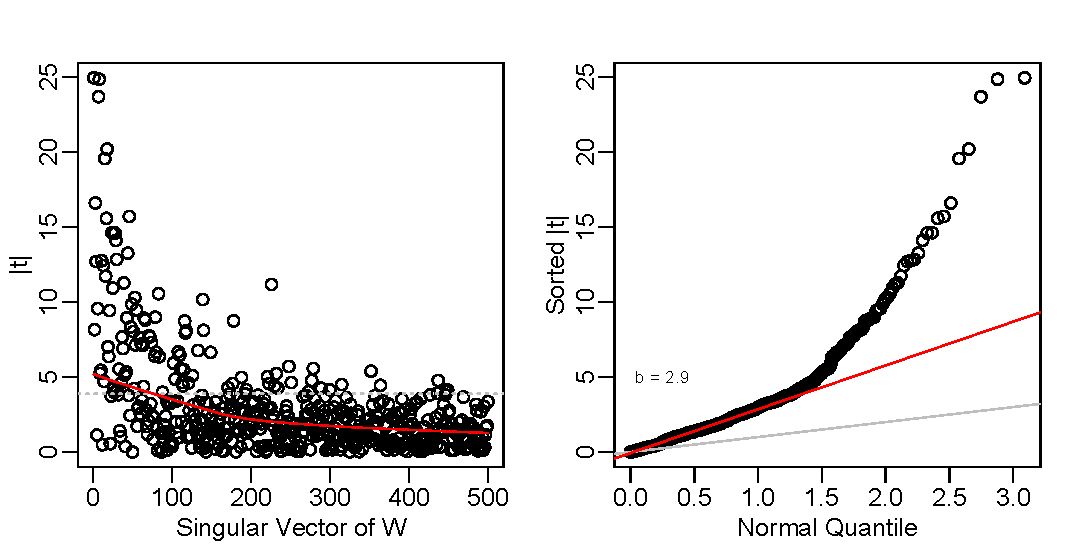
\includegraphics[width=6in]{figures/regrW}  }
 \centerline{  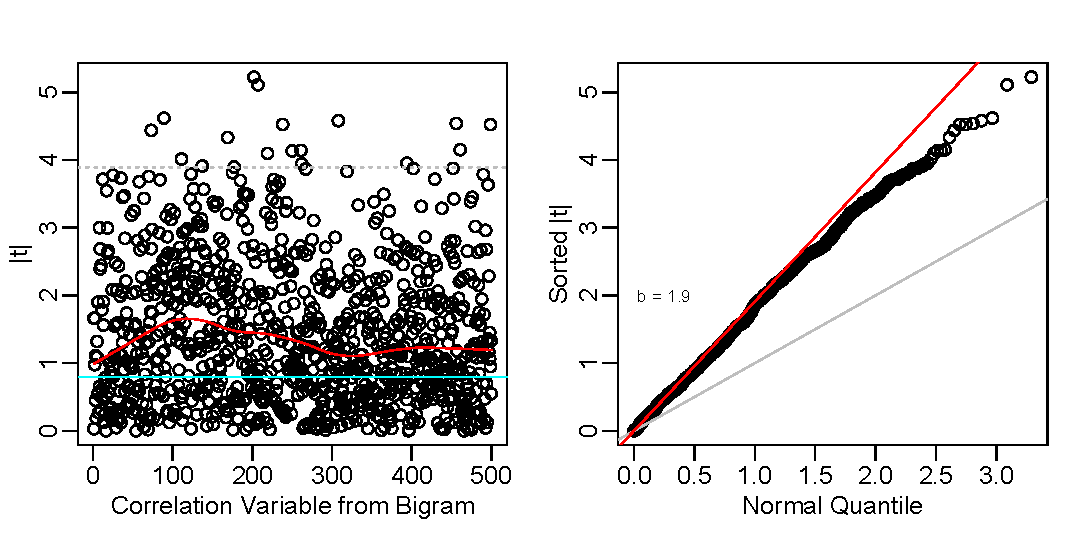
\includegraphics[width=6in]{figures/regrB}  }
 \end{figure}


\begin{table}
\caption{ \label{tab:regrB} {\sl Multiple regression of log prices on regressors derived from the bigram matrix $B$.}  Each regression uses correlations derived from $k_B$ left and $k_B$ right singular vectors.  }
\begin{center}
\begin{tabular}{ccccc}
	$2\,k_B$   & Residual SD &  $F$ & $R^2$  & $\ol{R}^2$  \cr
	200           &  0.842           &  40.0 &  0.527 &  0.514 \cr
	400           &  0.779           &  26.8 &  0.605 &  0.583 \cr
	600           &  0.750           &  20.6 &  0.645 &  0.614 \cr
	800           &  0.724           &  17.4 &  0.679 &  0.640 \cr
	1000         &  0.704           &  15.3 &  0.705 &  0.660
\end{tabular}
\end{center}
\end{table}


We can remove some of the effects of collinearity with a canonical correlation analysis.  Figure \ref{fig:cca} shows the canonical correlations between  $C_l$ and $C_r$.  The correlations remain close to 1 for about the first 100 or so canonical variables.  Rather than use the columns of $C_l$ as regressors, we can use the columns of the canonical variables from this analysis.  Figure \ref{fig:regrBcca} summarizes the estimates using the 500 predictors.  The regression signal is now much more concentrated in the initial canonical variables.  The overall fit, of course, matches that obtained by using $C_l$ directly since the canonical vectors are linear transformations of $C_l$.
 
 
 \begin{figure}
 \caption{ \label{fig:cca} { \sl Canonical correlations between the 500 columns of $C_l$ and $C_r$.} $C_l$ and $C_r$ project the left and right singular vectors of the bigram matrix into $\R^n$.}

 \centerline{
 \vspace{0.1in}
 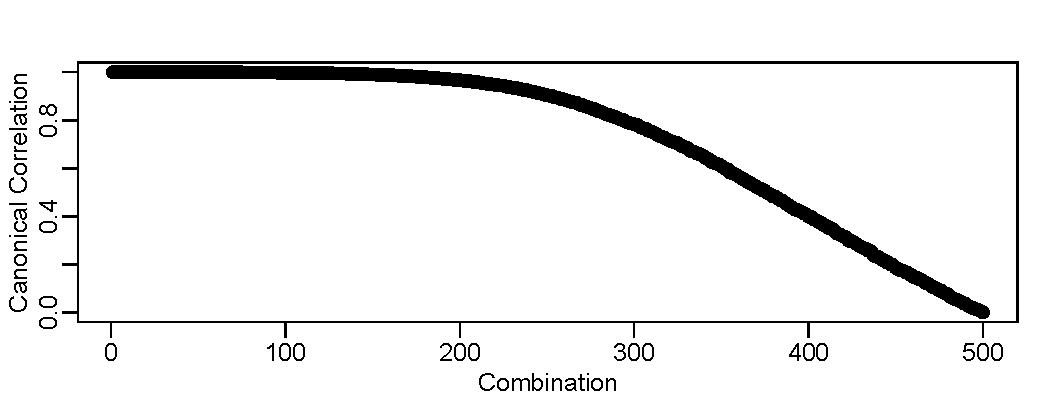
\includegraphics[width=3in]{figures/cca}  }
 \vspace{0.2in}
 \end{figure}


 \begin{figure}
 \caption{ \label{fig:regrBcca} { \sl Canonical variables from the analysis of the dependence between $C_l$ and $C_r$ concentrate more signal into the leading regressors.}}

 \centerline{
 \vspace{0.1in}
 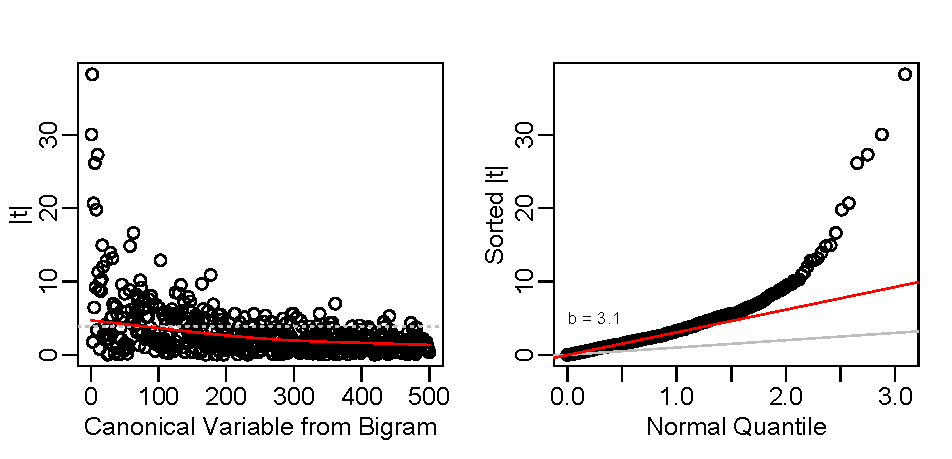
\includegraphics[width=5in]{figures/regrBcca}  }
 \vspace{0.2in}
 \end{figure}


How well do both sets of variables work?  To find out, we start with the variables from the LSA, the singular vectors of $W$.   The regression on the 500 singular vectors in $U_W$ explains $\ol{R}^2 = 0.612$ of the variation in log prices.  Adding the information from 500 more columns in $C_l$ boosts the total to $\ol{R}^2 = 0.679$.  Adding the remaining variation from $C_r$ raises the total slightly (albeit significantly) to $\ol{R}^2 = 0.703$. Interestingly,  the original parsed variables (Table \ref{tab:parsed}) offer ever so slightly more predictive power. The improvement only adds 0.003 to $\ol{R}^2$, but this is highly significant ($F$=12.1).



%--------------------------------------------------------------------------
\section{Motivating Probability Models}
\label{sec:model}
%--------------------------------------------------------------------------

 To provide some explanation for the evident success of this direct approach to building regressors from text, we offer a hypothetical data generating process for text and study the implications of this DGP for regression modeling.  The DGP is essentially that used in topic modeling \citep{blei12}.  In machine learning, topic modeling is an unsupervised technique that  clusters documents based on the presence of shared, underlying ``topics'' revealed by a hierarchical Bayesian  model.  Our method of featurizing text is also unsupervised,  but we seek to predict an explicit response rather than uncover latent clusters.  Nonetheless, we can study how our procedure would perform were there an underlying topic model.


\subsection {Topic Models}  % -------------------------------------------

 We begin with the simplifying assumption that real estate properties possess
 varying amounts of $K$ unobserved traits that influence both the value of
 a property as well as the language used to describe the property.  For example,
 such traits might include the quality of construction, presence of renovations,
 proximity to desirable conveniences and so forth.  In the context of topic models, these traits define the underlying topics shared by an ensemble of documents.  In what follows, the subscript $i$ indexes documents ($i = 1,\ldots,n$), $m$ denotes words ($m=1,\ldots,M$), and $k$ indexes traits ($k = 1,\ldots,K$).  Recall that words are tokens identified in the preprocessing of the text, not words in the usual sense.   Let $y = (y_1,\ldots,y_n)'$ denote the column vector that holds the response that is to be modeled by regression analysis.    In our application, $y$ is the vector of the log of prices of real estate. (All vectors are column vectors.)


 Within this model, traits influence the response via a familiar regression
 equation.  The connection between traits and documents is given by an unobserved $n \times K$ matrix of latent features $\zeta = [\zeta_{ik}]$.  Each row of $\zeta$ defines a mixture of traits that defines the distribution of words that appear in each document.  To avoid further notation, we use subscripts to distinguish the rows and columns of $\zeta$.  The vector $\zeta_{i*}$ identifies the row of $\zeta$ associated with document $i$, and $\zeta_{*k}$ identifies the column of $\zeta$ associated with topic $k$:
 \begin{displaymath}
   \zeta = \left( \begin{array}{c}
                    \zeta_{1*}' \cr \zeta_{2*}' \cr \vdots \cr \zeta_{n*}'
                  \end{array}
           \right) 
         = \left( \zeta_{*1} \; \zeta_{*2} \; \cdots \; \zeta_{*K} \right).
 \end{displaymath}
 $\zeta_{i*}$ specifies the distribution of traits present in the $i$th real-estate property; $0 \le \zeta_{ik} \le 1$ with $\sum_k \zeta_{ik} = 1$.  We assume that the allocation of traits within each document is an independent realization of a Dirichlet random variable, 
 \begin{equation}
  \zeta_{i*} \sim \mbox{Dir}(K, \al_K) \;,
  \label{eq:zeta}
\end{equation}
where $\al_m$ denotes the $K$-dimensional parameter vector of distribution.    Given $\zeta$, the $K$ traits  influence the response through a linear equation of the familiar form
 \begin{equation}
    \ev y_i = \zeta_{i*}' \, \beta \;.
 \label{eq:regr}
 \end{equation}
 The coefficients $\beta$ determine how the traits influence the response.  


 These traits also determine the distribution of words that appear in documents.  This connection allows us to recover $\zeta$ --- which is not observed --- from the associated text.  Assume that a trait defines a probability distribution over the word types in the vocabulary $V$.  Let $P_k$ denote the distribution of word-types used when describing trait $k$; in particular, $P_{km}$ is the probability of using word type $m$ when describing trait $k$.  Our DGP models these distributions over word types as another set of independent Dirichlet random variables,
 \begin{equation}
   P_k \sim \mbox{Dir}(M, \al_M),
   \label{eq:Pk}
 \end{equation}
where $\al_M$ is the $M$-dimensional parameter vector for the distribution.
 Collect these discrete
 distributions in the $K \times M$ matrix
 \begin{equation}
    P = \left(  \begin{array}{c} 
                    P_1' \cr P_2' \cr  \vdots \cr P_K'
                \end{array}
        \right) \;.
 \label{eq:P}
 \end{equation}
 
 
The Dirichlet variables $\zeta$ and $P$ together determine a distribution for the counts of words that appear in each document (its bag-of-words).  First, we assume that the number of words in each document is another independent random variable, and for our simulation we use a negative binomial, formed by mixing Poisson distributions with parameters that have a Gamma distribution,
\begin{equation}
  m_i|\la_i \sim \mbox{Poisson}(\la_i), \quad \la_i \sim \mbox{Gamma}(\al),
\end{equation}
independently over documents.  To `construct' the $i$th document from this model, we sample $m_i$ words from the underlying $K$ topics by the following mechanism.  Let $w_{im}$ denote the $m$th word in the $i$th document.  For this word, pick a topic at random (and independently) from the topic distribution identified by $\zeta_{i*}$, say $k_{im} \sim \mbox{Multi}(\zeta_{i*})$.  Then choose $w_{im}$ from the multinomial distribution with these probabilities, 
\begin{equation}
  w_{im} \sim \mbox{Mult}(P_{k_{im}}), \quad i = 1,\ldots,m_i \;.
  \label{eq:wim}
\end{equation}
Hence, the vector of counts $w_i$ for the $i$th document has a multinomial distribution whose parameters are determined by its mixture of traits:
 \begin{equation}
   w_i' \sim \mbox{Multi}(m_i, \zeta_i' P)   
 \label{eq:di}
 \end{equation}
 implying that $\ev w_i' | m_i = m_i \; \zeta_i'P$.  
 
 \remark{ According to this DGP, the length of a document $m_i$  does not affect the response; only the mixture of traits is relevant.  Our results with real text summarized in the regression (Table \ref{tab:parsed}) provide contradictory evidence: Document length has a significant impact on price. }
 
 
   Given that documents are generated by a topic model defined by equations \eqn{eq:regr} -- \eqn{eq:di}, the challenge for making regression features from text is to recover the $K$-dimensional linear space spanned by $\zeta$.  The success of latent semantic analysis (LSA, principal components analysis of the word counts $W$) is particularly easy to see. Intuitively, LSA is well-matched to this DGP because both treat a document as a bag-of-words.  Let $D_m$ denote an $n \times n$ diagonal matrix with the  word counts $m_i$ along the diagonal.  Then the expected value of the document/word matrix $W$ is the sum of $K$ outer products:
\begin{equation}
    \ev W = D_m \; \zeta \; P = D_m \sum_k \zeta_{*k} P_k' \;.
  \label{eq:EW}
\end{equation}
The expectation factors as an outer product, just as an SVD represents a matrix. That is, if we write $X = UDV'$, then we can express the matrix product as the sum $X = \sum_j d_{jj} u_j v_j'$ where $u_j$ and $v_j$ are the columns of $U$ and $V$, respectively.  For our models of text, the left singular vectors $U_W$ from \eqn{eq:svdW} are related to the allocation of traits over documents held in $\zeta$.  Of course, there are many ways to factor a matrix, and it is not apparent why the factorization provided by the SVD would be better than others.  Our rationale relies on convenience (and the evident success in modeling real-estate prices), but one can argue that a decomposition that yields positive factors, namely non-negative matrix factorization NMF, would be more appropriate. Because both $\zeta$ and $P$ are probability matrices, a constrained optimization that factors $W$ into matrices whose rows are discrete probability distributions would be ideal.   We do not explore these here. 


\remark{ Expression \eqn{eq:EW} suggests that we should factor out $D_m$ from $W$ before doing the singular value decomposition so that variation of the lengths $m_i$ does not contaminate the left singular vectors.  This replacement of counts by proportions would then be followed by weighted least squares to down weight the influence of short documents.  We explored several variations of this weighting, but none made a dramatic difference in the goodness of fit or out-of-sample accuracy. }


The connection of this DGP to bigrams is less obvious and relies more on stronger assumptions.  Bigrams count the frequency of the adjacent word types, a property we associate with the sequence of words rather than co-occurrence within a document.  To see how the analysis of bigrams can nonetheless produce useful regressors, we need to add either stronger assumptions to our DGP or incorporate some type of sequential dependence.  For example, we might assume that words associated with traits appear in {\em phrases}.   As in the bag-of-words model, words within a phrase are drawn independently from the distribution defined by a trait, but the generating process samples within a trait for some length of time before transitioning to another trait (resembling an HMM).  If these phrases are relatively long, then we can approximate the expected counts in the bigram matrix as a weighted outer product of the probability vectors for the traits.  We can obtain the same heuristic in our DGP by assuming that the probability distributions $P_k$ that define the traits have (nearly) singular support on words.  That is, most words are associated with a unique trait (implying $P_{k_1}'P_{k_2}  \approx 0$).  In either case, the marginal probability of finding adjacent words types reveals the underlying probability distribution.  


For instance, suppose the traits have disjoint support on words and that documents have common length $m_i \equiv m$. Then the probability of finding  word types  $w_{m_1}$ and $w_{m_2}$ from trait $k$ adjacent to each other is 
 \begin{equation}
  P(w_{m_1},w_{m_2}) = \sum_i \left(\zeta_{ik}^2/n \right) P_{km_1} P_{km_2} 
                                     = h_k P_{km_1} P_{km_2}  \;.
  \label{eq:joint}
\end{equation}
Let $N = \sum m_i$ denote the total number of observed words. Using the expression \eqn{eq:joint}, the expected value of the bigram matrix factors as
 \begin{equation}
    \smfrac{1}{N} \ev B \approx \sum h_k P_k\; P_k' = P' H P \;, 
                     \qquad  H = \mbox{diag}(h_k)\;,
 \label{eq:B2}
 \end{equation}
Again, a constrained factorization that produced probability vectors would be more appropriate if one truly believed this model.  In an ideal world, the singular values of the SVD would capture the unobserved marginal probabilities  $h_k$.  Expression \eqn{eq:B2} also suggests why the left and right singular vectors of $B$ should match, or at least define a common subspace.


 The factorization of $B$ defines the coordinates of eigenwords ($\R^M$).  To
 obtain coordinates in document space ($\R^n$) for use in regression, we  correlate  the word counts in $W$ with the eigenwords.  For the $i$th description, if we pretend that the factorization of $B$ is exact and approximate the word counts $w_i$ by their expectation, then the first column of $w_i' U_b$ is
 \begin{displaymath}
    w_i'P_1 \approx m_i \zeta_i' P P_1 \;.
 \end{displaymath}
 If the probability distributions of the traits are roughly singular as argued previously, then
 \begin{displaymath}
    w_i'P_k \approx m_i \zeta_{i1} P_1'P_1 \;.
 \end{displaymath}
 Hence, to this rough approximation, the correlation between $w_i$ and the first
 left singular vector of $B$ is
 \begin{displaymath}
    \corr(w_i, U_{B1}) = \frac{\zeta_{i1}}{(\zeta_{i*}'\zeta_{i*})^{1/2}}   
 \end{displaymath}
 The L2 normalization is just right for canceling $P_1$, but leaves a constant
 factor $\norm{\zeta_i}$.

 
 Of course, even in expectation, the factorization of the bigram $B$ will not
 match  \eqn{eq:B2}; the SVD  only recovers a basis for the range of $B$.  Thus, the 
 singular vectors will mix the probability vectors.  We can
 then think about $U_B = P'O$ for some orthonormal matrix $O$.  That is, ideally
 the singular vectors span the correct space, but in a different basis so that
 we observe (again, in expectation)
 \begin{displaymath}
   w_i'U_b \approx (m_i \zeta_i'P)(P'O) = m_i \zeta_i \mbox{diag}(P_k'P_k) O
 \end{displaymath}
 Hence, when computing the correlations between the observed counts $w_i$ and the
 singular vectors, the norm of the probability distributions cancel and we
 obtain a rotation of  $\zeta_{i*}$ vector.  The rotation is the same, however,
 for all rows, and consequently our collection of regressors spans the same
 space as the unrotated $\zeta$.


 Obtaining a the relevant $\zeta$-coordinates for a new document is routine in
 this case.  One simply mimics the process used to identify/estimate $\zeta$ for
 the observed cases by correlating the counts for the new description, say
 $w_{new}$, with the matrix defined by the eigenwords.



%--------------------------------------------------------------------------
\subsection{Examples: Simulated Data from Topic Models}

 To get a better handle on how the singular value decomposition works, consider
 a simulated world in which a topic model generates text from a vocabulary of $M
 = 2,000$ words types.  Assume that words in $n = 6,000$ documents are generated by mixture of $K=10$ topics, with each topic defined by  one of $K$ distributions $P_1,\ldots, P_{10}$ over the 2,000 word types.  
 Hence, $p_1$ lies in the $M$-dimensional
 simplex.     Similarly, the distribution of topics within the $i$th document is distributed as $\zeta_{i*} \sim \mbox{Dirichlet}(K, \al_k=0.1)$.  The response for a document is a weighted sum of the mix of topics within the document.  We consider two situations, first the idealized case in which topic distributions are essentially disjoint, and then with topic distributions share common words.
 
 \subsubsection{Nearly Disjoint Topic Distributions} % -----------------
 
  
 For this example, we simulate $P_k$ by independently drawing from a Dirichlet distribution with parameters $M$ and $\al_m = 0.05$ for all $m = 1,\ldots,M$.  Small values of $\al_m$ lead to `spiky' distributions with little overlap.  For example, Figure \ref{fig:simdist}(a) graphs the probabilities assigned by two of the 10 distributions for this first simulation.  The defining constants for this first example are:
 \begin{displaymath}
    M = 2000 \mbox{ word types}, \quad
    n = 4000 \mbox{ documents},  \quad
    K = 10 \mbox{ topics}   
 \end{displaymath}
 with random variables defined by
 \begin{eqnarray*}
    m_i           &\sim& \mbox{Pois}(\la_i), \la_i \sim \mbox{Gamma}(30,1)\;,
                     i = i,\ldots, n, \quad \mbox{ (Negative Binomial) }       \cr
    P_k                &\sim& \mbox{Dir}(M, \al_m=0.05), \quad k=1,\ldots,K,  \cr
    \zeta_{i*}        &\sim& \mbox{Dir}(K, \al_k=0.10),\quad i=1,\ldots,n,  \cr
    k_{im}             &\sim& \mbox{Mult}(\zeta_{i*}), \quad m=1,\ldots,m_i,    \cr 
    w_{im}|k_{im} &\sim& \mbox{Mult}(P_{k_{im}}), \quad i=1,\ldots,n \;, \cr
    y_i                  &\sim& N(\zeta'\beta, 0.5^2), \quad i = 1,\ldots,n \;.
 \end{eqnarray*}
 With these choices, $\ol{R}^2 \approx 0.92$ for the regression of $y$ on $\zeta$.

 
\begin{figure}
 \caption{ \label{fig:simdist}
  \sl Probabilities assigned to words by two simulated topic distributions with (a) nearly disjoint support and (b) with overlapping words.}  
  \centerline{   
     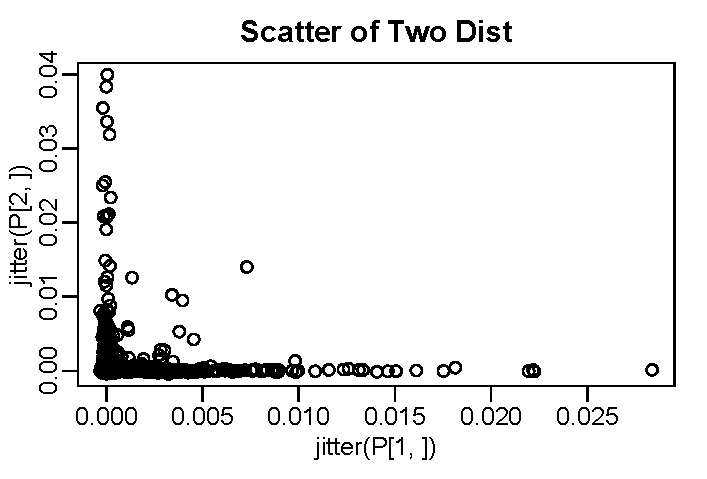
\includegraphics[width=3in]{figures/simdist}    
     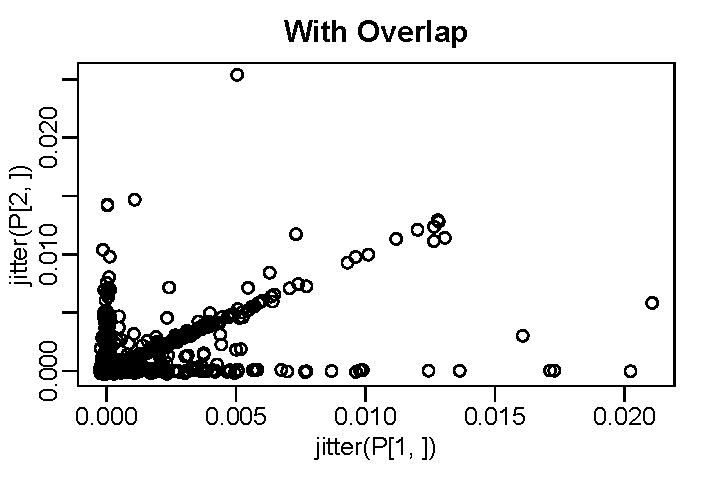
\includegraphics[width=3in]{figures/simdistB}    }
\end{figure}


The distribution of words produced by this topic model  loosely resembles the distribution found in real estate ads.  Compare Figure \ref{fig:simzipf}(a) to Figure \ref{fig:zipf} from the real estate data.  Though a good match for the less common words, the most common words are not as common as one might want.  The common words do not have a high enough frequency (disjoint topics lack common words like `a' and `the' and punctuation as found in the real-estate listings shown in Figure \ref{fig:zipf}), and the frequencies for rare words drop off too quickly.  


\begin{figure}
\caption{ \label{fig:simzipf} { \sl Distribution of word frequencies for simulated
topic data, based on (a) disjoint word distributions and (b) over-lapping distributions.}}
 \centerline{
 \vspace{0.1in}
 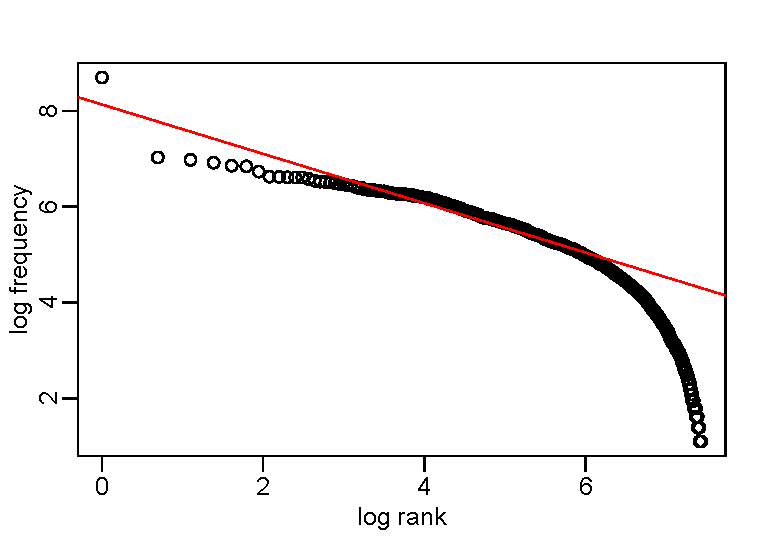
\includegraphics[width=2.5in]{figures/simzipfA}  
 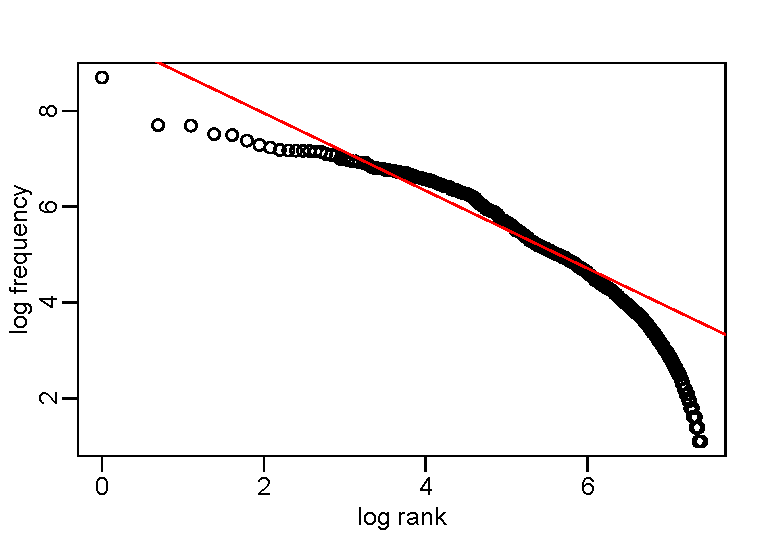
\includegraphics[width=2.5in]{figures/simzipfB} }
  \vspace{0.2in}
 \end{figure}


Table \ref{tab:simregr} summarizes the fits using $k_W = 100$ singular vectors and $k_B=100$ left and right singular vectors of $B$.  The fits recover much, but certainly not all of the underlying regression structure (for which $R^2 \approx 0.92$).  The fitted models produce similar fitted values, as shown in Figure \ref{fig:simfits}.  The two fits, however, deviate for documents with either lower or higher values of $y$. \ras{ Would measurement error produce this tail curvature?}

\begin{table} 
\caption{ \label{tab:simregr}
\sl Fits to regression in simulated topic data using singular vectors of $W$ and $B$ for two topic distributions.}
\begin{center} 
\begin{tabular}{|c|ccc|}
\hline
  Topic Structure & Num Regressors & Origin & $\ol{R}^2$ \cr \hline \hline
   Disjoint            &         100              &  $W$  &  0.746        \cr
                           &         200              &  $B$  &   0.788        \cr \hline \hline
   Overlapping    &          100              &  $W$ &   0.516       \cr
                           &          200             &  $B$  &   0.626        \cr \hline
\end{tabular}
\end{center}
\end{table}


\begin{figure}
\caption{ \label{fig:simfits}  
{\sl Scatterplot of fitted values for the two regressions based on singular vectors of $W$ and $B$.}  The shown smooth curve is the lowess fit, and the correlation $r \approx 0.97$.}
\centerline{  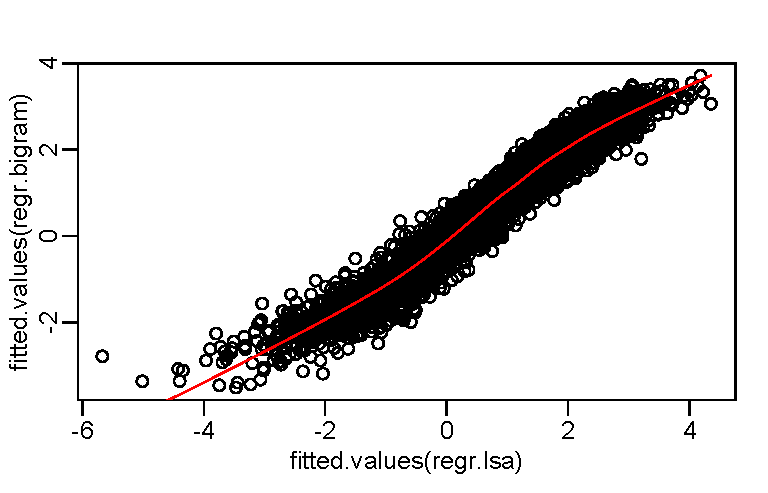
\includegraphics[width=4in]{figures/simfits}  }
\end{figure}


Because the topic distributions are nearly disjoint, one can identify the number of topics $K$ from the singular value decompositions.  The value of $K$ is most apparent in a canonical correlation analysis of the singular vectors of $B$.  Figure \ref{fig:simccab} graphs the canonical correlations for the left and right singular vectors
of the bigram matrix for the simulated text.  The clear break in the sequence of singular vectors confirms the presence of $K=10$ topics.  

 \begin{figure}
  \caption{ \label{fig:simccab} { \sl Canonical correlations for left and right
 singular vectors of the bigram matrix $B$ of simulated topic data.} (a) The underlying topics are nearly disjoint in support. (b) The underlying topics overlap.}
\vspace{0.1in}
 \centerline{
      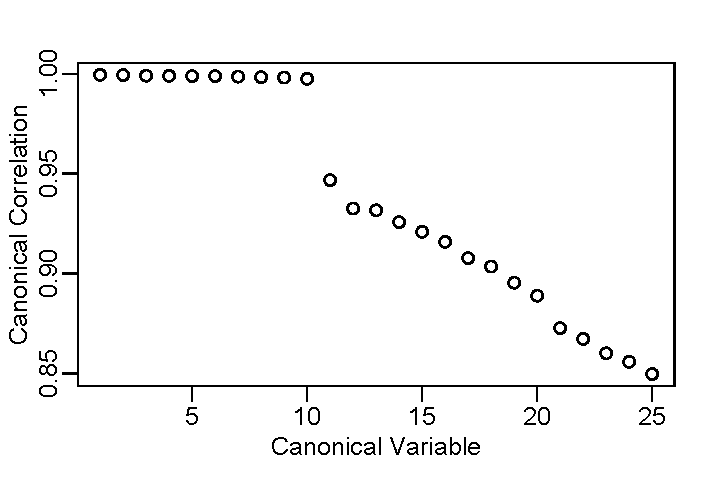
\includegraphics[width=3in]{figures/simccab}  
      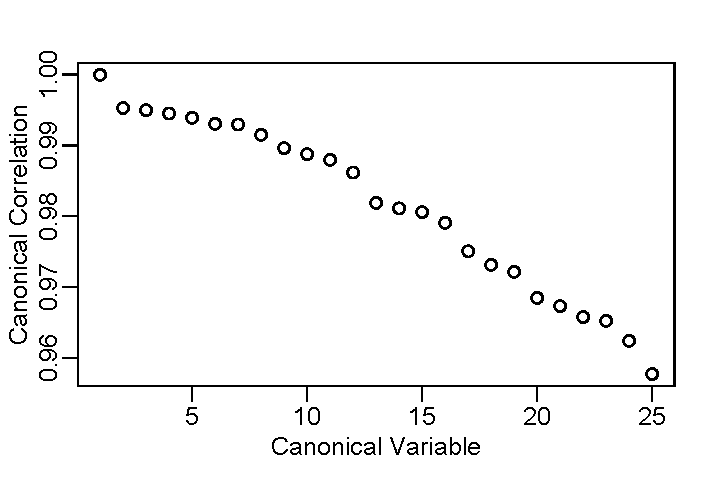
\includegraphics[width=3in]{figures/simccabb}   }
  \end{figure}
 
 
 \subsubsection{Overlapping Topic Distributions} % -----------------
 
 The ability to recover the underlying regression structure is diminished in the presence of overlapping topics.  The simulation in this section is virtually identical to the previous one, but for overlapping topics.  The simulation again has a vocabulary of $M=2,000$ words, $n=6,000$ documents, and $K=10$ topics.  Rather than simulate the topics distributions independently, however, we introduce a common structure.  The topic distributions share 150 ``common words'' that follow with probabilities from a Dirichlet distribution.  Let $X \sim \mbox{Dir}(150, 2)$ and let $\xi$ denote the vector obtained by concatenating $M$ - 150 zeros onto $X$, $\xi' = (X, 0 , \ldots, 0)$.  The distribution that defines the $k$th trait is then $P_k = \xi/2 + Z/2$ with $Z \sim \mbox{Dir}(\al_m)$.  Figure \ref{fig:simdist}(b) plots the probabilities of two distributions generated in this manner.  The diagonal points show the substantial overlap.  The number of topics per document and the marginal distribution of words per document are both similar to the prior simulation and are not materially influenced by the introduction of this overlap.
 
 
 The same cannot be said for the regressors produced from singular value decompositions.  The lower portion of Table \ref{tab:simregr} summarizes these fits.  The regression on 100 singular vectors from $W$ now captures $\ol{R}^2 = 0.516$ of the variation in the response, and the regressors from the bigram obtain $\ol{R}^2 = 0.626$.  The correlation between fitted values falls to 0.86 (down from 0.97 when no overlap was introduced).  Curiously, the bigram is less influenced by the overlap.  
 Canonical correlation of the singular vectors of $B$ also no longer reveals the number of topics (Figure \ref{fig:simccab}(b)).   The canonical correlations between left and right singular vectors of $B$ now provide no hint as to the choice of $K$.  
 
 
 Figure \ref{fig:simregr} summarizes the statistical significance of the coefficient estimates in this model.  The distribution of significance is rather different from that seen in the real estate models (Figure \ref{fig:svdregr}).  For example, statistical significance decays in the real estate model as one moves from the leading singular vectors of $W$ down to smaller vectors.  The simulated results show no hint of greater significance in the leading singular vectors.  \ras{That surprised me.}
  Also, both half-normal plots are very nearly linear, with little of the ``superstar'' character seen in the $t$-statistics from the regression models for real estate.  What is similar to the model for prices is that the signal is more diffuse in the regression using correlation regressors derived from $B$.  The slope of the line fitted to the half-normal plot of the $t$-statistics for the singular vectors of $W$ is 8.8, whereas that for the regressors derived from $B$ is 3.6.  
 
 
 \begin{figure}
 \caption{ \label{fig:simregr}
  {\sl Distribution of statistical significance in the regression with simulated, overlapping topic models.} Results first for the regression on singular vectors from $W$, then those derived from the bigram matrix $B$.}
   \centerline{ 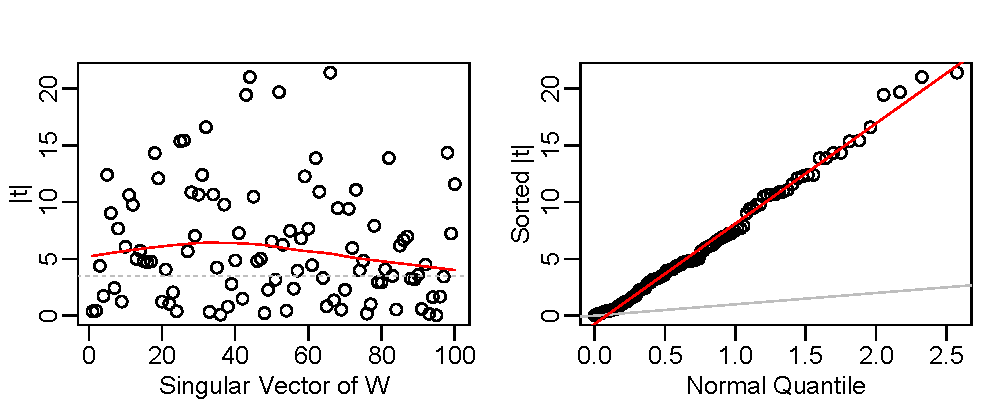
\includegraphics[width=5in]{figures/simregrW}  }
   \centerline{ 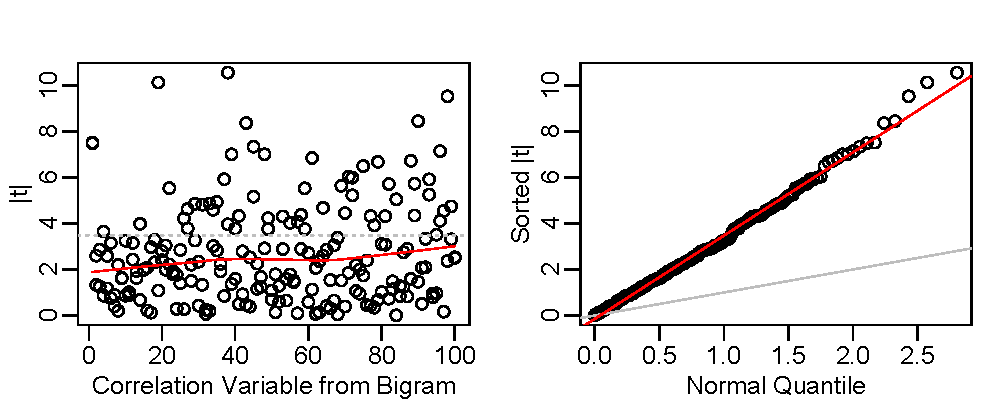
\includegraphics[width=5in]{figures/simregrB}  }
 \end{figure}

%--------------------------------------------------------------------------
\section{Variable Selection and Cross Validation}
\label{sec:cv}
%--------------------------------------------------------------------------

Transductive case, rather than so-called inductive case.

%--------------------------------------------------------------------------
\section{Lighthouse Variables and Interpretation}
\label{sec:light}
%--------------------------------------------------------------------------
 
 Though regression models are seldom causal, one is often tempted to interpret
 properties of the solution within the domain of application.  Because the
 predictors computed from the decompositions in the prior section describe
 subspaces rather than some specific property of words, interpretation is
 essentially non-existent.


 To obtain features that are interpretable, we exploit the presence of
 concrete features that are occasionally observable.  For example,
 most home listings do not include the number of square feet.  An
 explanatory variable obtained by parsing the $s_i$ is missing most
 values.  We can use this variable, however, to construct a more
 interpretable variable from $U_G$ and $H$.  


 Let $z \in \Rn$ denote the partially observed or perhaps noisy data
 that measures a substantively interesting characteristic of the
 observations.  Rather than use $z$ directly as a predictor of $y$, we
 can use it to form an interpretable blend of $U_G$ and $H$.  In
 particularly, we simply regress $z$ on these columns, finding the
 linear combination of these matrices most correlated with the
 observed information.  This variable, call it $\hat{z}$ then becomes
 another regressor.  Because we use such variables to guide the
 construction of interpretable combinations of the bases $U_G$ and
 $H$, we call these lighthouse variables.



%--------------------------------------------------------------------------
\section{Next Steps}
\label{sec:disc}
%--------------------------------------------------------------------------
  
 \begin{itemize}
 
 \item The initial regression on words is not nearly black.

 \item Cross validation, prediction on hold-out.  (Such as for the more recent data, as a very simple sort of illustration of partial transfer learning.)
 
 \item Comparison to Google predict.  What do they do behind the curtains?
 
 
 \item Further work:
   \begin{description}
   
   \item[Other domains.]  We have applied these same methods to similarly structured data from other domains.  For example, we built a regression to predict the ratings of wine using variables constructed from the SVDs of $W$ and $B$ for about 21,000 ratings of wine.  Though a larger number of documents, these descriptions are shorter (averaging 42 words).  The qualitative properties of our example with real estate carries over to that modeling.  For instance, plots of the coefficients share the features shown in Figure \ref{fig:svdregr}: A greater concentration in the LSA variables with the signal widely spread over coordinates.  The fits for the wine ratings are stronger, however.  Using the first 100 LSA singular vectors produces $\ol{R}^2 = 0.61$.

   \item[Transfer learning.]  Going from one location (Chicago) to another.
   
   \item[Use of unsupervised data.] such as google eigenwords.
   
   \item[n-grams.]  Can use trigrams or skipped bigrams.
   
   \item[Variable selection.]  In particular, nonlinear variables -- namely interactions -- or the use of other n-grams rather than just bigrams.  Perhaps some shrinkage as well to improve predictions.  Alpha investing results.
   
 \item[More elaborate tokenizing] Would be interesting to explore the use of stemming to reduce the number of word types and with a larger collection of documents, to explore annotation (that would distinguish words by their part of speech).  Further parsing, lexical analysis.  Some readers will be troubled by the simplicity of the  ``bag-of-words'' representation of a document.  Our methods understand neither English nor the rules of grammar or spelling, nor do they attempt to untangle the multiple uses of the same word.  Linguists have debated the ability of such  representations to reveal the meaning of language, and it is clear that the bag of words representation loses information.  Just imagine cooking from "bag of words" recipe or following a "bag of words" driving directions.  Nonetheless, this very direct representation produces very useful explanatory variables within our application.  We leave open the opportunity to embellish this
 approach with more domain specific methods of parsing, such as adding
 part-of-speech tags and lexical information.

   \end{description}

\end{itemize}


%--------------------------------------------------------------------------
\section*{Acknowledgement}
%--------------------------------------------------------------------------

The authors thank Vanessa Villatoro from Trulia's PR Team for allowing us to scrape the data from their web site.


%--------------------------------------------------------------------------
% References
%--------------------------------------------------------------------------

\bibliography{../../../references/stat,../../../references/TextPapers/text}
\bibliographystyle{../bst/ims}

\end{document} %==========================================================
